% !TeX root = main.tex

\hypertarget{rules-of-derivatives}{%
\section{Rules of Derivatives}\label{rules-of-derivatives}}

\hypertarget{basic-rules}{%
\subsection{Basic Rules}\label{basic-rules}}

\textbf{The Constant Rule:} Let \(c\) be a constant number. Then
\[\frac{\mathrm{d}}{\mathrm{d}\,x}(c)=0.\]

\textbf{The Power Rule:} Let \(n\) be a positive integer. Then
\[\dfrac{\mathrm{d}}{\mathrm{d}\,x}\left(x^n\right)=nx^{n-1}.\]

\begin{example}
Let \(f(x)=x^4\). Find \(f'(x)\).
\end{example}
\vspace*{6\baselineskip}

\hypertarget{linear-combination-rules}{%
\subsection{Linear Combination Rules}\label{linear-combination-rules}}

Let \(f\) and \(g\) be differentiable functions. Let \(a\) and \(b\) be
two constant numbers. Then \[\big(af+bg\big)'(x)=af'(x)+bg'(x).\]

\begin{example}
Let \(f(x)=4x^5-3x^2+7\). Find \(f'(x)\)
\end{example}
\vspace*{6\baselineskip}

\hypertarget{the-product-and-quotient-rules}{%
\subsection{The Product and Quotient
Rules}\label{the-product-and-quotient-rules}}

\textbf{Product Rule:} Let \(f\) and \(g\) be differentiable
functions. Then \[
(f\cdot g)'(x)=f'(x)g(x)+f(x)g'(x).
\]


\begin{example}
Find the derivative of the function \(f(x)=(x^3-2x+1)(x^2-3x+5)\).
\end{example}
\vspace*{6\baselineskip}

\begin{example}
For \(p(x)=f(x)g(x)\), use the product rule to find \(p'(2)\) if
\(f(2)=3,\; f'(2)=-4,\; g(2)=1\), and \(g'(2)=6\).
\end{example}
\vspace*{6\baselineskip}

\textbf{The Quotient Rule:} Let \(f\) and \(g\) be differentiable
functions. Then
\[\left(\dfrac{f}{g}\right)'(x)=\dfrac{f'(x)g(x)-f(x)g'(x)}{(g(x))^2}.\]

\begin{example}
Find the derivative of the function \(f(x)=\dfrac{x^2-3x}{3x-5}\).
\end{example}
\vspace*{6\baselineskip}

\begin{example}
Let \(f=\dfrac{g}{x^2+1}\) where the graph of the function \(g\) is
given below. Find \(f'(2)\).\\
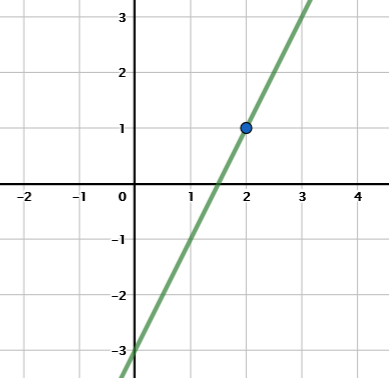
\includegraphics[width=0.8\textwidth]{img/quotientRuleLinear.png}
\end{example}
\vspace*{6\baselineskip}

\hypertarget{extended-power-rule}{%
\subsection{Extended Power Rule}\label{extended-power-rule}}

Let \(k\) is a real number. Then
\[\dfrac{\mathrm{d}}{\mathrm{d}\,x}(x^k)=kx^{k-1}.\]

If \(k\) is a negative integer, the formula follows from the quotient
rule. The proof of the general cases has to be postponed after
logarithmic and exponential functions in Calculus II.

\begin{example}
Find \(\dfrac{\mathrm{d}}{\mathrm{d}\,x}(x^{-5})\).
\end{example}
\vspace*{6\baselineskip}

\begin{example}
Find \(\dfrac{\mathrm{d}}{\mathrm{d}\,x}\dfrac{1}{\sqrt[3]{x}}\).
\end{example}
\vspace*{6\baselineskip}

\hypertarget{example-and-practice-on-differentiation-rules}{%
\subsection{More Examples and Practice}\label{example-and-practice-on-differentiation-rules}}

\begin{example}
Let \(f(x)=3x^2h(x)+\dfrac{g(x)}{x}\). Find \(f'(x)\) in terms of \(h\),
\(g\), \(h'\) and \(g'\).
\end{example}
\vspace*{6\baselineskip}

\begin{example}
Determine the values of \(x\) for which \(f(x)=x^3-7x^2+8x+1\) has a
horizontal tangent line.
\end{example}
\vspace*{6\baselineskip}

\begin{example}
Find equations of the normal line to the curve \(y=4\sqrt{x}-x\) at
\((1,3)\).
\end{example}
\vspace*{6\baselineskip}

\subsection{Practice}

\begin{exercise}
  Let \(f(x)=x^{11}\). Find \(f'(x)\).
  \end{exercise}
  \vspace*{6\baselineskip}
  
\begin{exercise}
Let \(g(x)=5x^{10}-5x^3-9\). Find \(g'(x)\).
\end{exercise}
\vspace*{6\baselineskip}

\begin{exercise}
Find the equation of the line tangent to the graph of \(f(x)=x^2-4x+6\)
at \(x=1\).
\end{exercise}
\vspace*{6\baselineskip}

\begin{exercise}
Let \(h(x)=f(x)(x^3-3x^2-2x)\) where \(f\) is differentiable, \(f(1)=2\)
and \(f'(1)=3\). Find \(h'(1)\).
\end{exercise}
\vspace*{6\baselineskip}

\begin{exercise}
Find \(h'(x)\) for \(h(x)=\dfrac{1}{x^5}\).
\end{exercise}
\vspace*{6\baselineskip}

\begin{exercise}
Let \(f\) and \(g\) be differentiable functions such that \(f(3)=2\),
\(f'(3)=-1\), \(g(3)=-2\) and \(g'(3)=1\). Find the \(h'(3)\) where
\(h(x)=\dfrac{f(x)-2}{g(x)}\).
\end{exercise}
\vspace*{6\baselineskip}

\begin{exercise}
Find the derivative of the function \(f(x)=\dfrac{1}{\sqrt[7]{x^3}}\).
\end{exercise}
\vspace*{6\baselineskip}

\begin{exercise}
  Find \(g'(x)\) for
  \(g(x)=\frac{3x^2+5x-7}{\sqrt{x}}\).
\end{exercise}
\vspace*{6\baselineskip}

\begin{exercise}
Let \(h(x)=\dfrac{2x^3f(x)}{3x+g(x)}\). Find \(h'(x)\) in terms of
\(f\), \(g\), \(f'\) and \(g'\).
\end{exercise}
\vspace*{6\baselineskip}

\begin{exercise}
Determine the values of \(x\) for which \(f(x)=2x^3-5x^2-x+7\) has a
tangent line parallel to \(y=3x-1\).
\end{exercise}
\vspace*{6\baselineskip}

\begin{exercise}
Suppose that \(f\) and \(g\) are both differentiable functions with
\(f(4)=3\), \(g(4)=2\), \(f'(4)=9\) and \(g'(4)=5\). Find \(h'(4)\)
where \[
h(x)=\frac{2}{\sqrt{x}}-\frac{f(x)-1}{g(x)}.
\]
\end{exercise}

